In this lecture, we introduce the language of quantum computing: qubits and Dirac (bra-ket) notation,
unitary matrices, and quantum circuits. We meet the gates $X$, $H$ and CNOT, define the tensor product
that combines several qubits into one state, and show that some two-qubit states are entangled.

\section{Qubits}

A classical \emph{bit} takes one of the two values $0$ and $1$. A quantum bit can be in a combination
of both.

\begin{definition}[Qubit, $n$-Qubit State]\label{def:qubit-0915}
    The state of one \textbf{qubit} is a unit vector in $\mathbb{C}^2$,
    \[\begin{pmatrix} \alpha \\ \beta \end{pmatrix}
        = \alpha \begin{pmatrix} 1 \\ 0 \end{pmatrix} + \beta \begin{pmatrix} 0 \\ 1 \end{pmatrix}
        = \alpha \ket{0} + \beta \ket{1},
        \qquad \abs{\alpha}^2 + \abs{\beta}^2 = 1,\]
    where $\ket{0} = \begin{pmatrix} 1 \\ 0 \end{pmatrix}$ and
    $\ket{1} = \begin{pmatrix} 0 \\ 1 \end{pmatrix}$ form the \textbf{computational basis}. The
    complex numbers $\alpha, \beta$ are the \textbf{amplitudes}. More generally, the state of $n$
    qubits is a unit vector in $\mathbb{C}^{2^n}$,
    \[\ket{\phi} = \sum_{x \in \set{0,1}^n} \alpha_x \ket{x},
        \qquad \sum_{x \in \set{0,1}^n} \abs{\alpha_x}^2 = 1,\]
    where $\ket{x}$ is the standard basis vector with a $1$ in the position indexed by the bit string
    $x$ (the $2^n$ strings are listed in increasing binary order) and $0$ elsewhere. Measuring the
    state gives the outcome $x$ with probability $\abs{\alpha_x}^2$.
\end{definition}

For one qubit, a measurement gives $0$ with probability $\abs{\alpha}^2$ and $1$ with probability
$\abs{\beta}^2$; the normalization says exactly that these probabilities sum to $1$. In short,
``amplitude $= \sqrt{\text{probability}}$'': the modulus of an amplitude is the square root of the
corresponding probability.

\paragraph{Remark.} On the board the normalization was written as $\sqrt{\alpha^2 + \beta^2} = 1$.
Since the amplitudes are complex, the squares must be squared moduli, as in \cref{def:qubit-0915}.

\paragraph{Two qubits.} The state of two qubits has four amplitudes, one for each of $00, 01, 10, 11$:
\[\begin{pmatrix} \alpha \\ \beta \\ \gamma \\ \delta \end{pmatrix}
    = \alpha \begin{pmatrix} 1 \\ 0 \\ 0 \\ 0 \end{pmatrix}
    + \beta \begin{pmatrix} 0 \\ 1 \\ 0 \\ 0 \end{pmatrix}
    + \gamma \begin{pmatrix} 0 \\ 0 \\ 1 \\ 0 \end{pmatrix}
    + \delta \begin{pmatrix} 0 \\ 0 \\ 0 \\ 1 \end{pmatrix}
    = \alpha \ket{00} + \beta \ket{01} + \gamma \ket{10} + \delta \ket{11},\]
with $\abs{\alpha}^2 + \abs{\beta}^2 + \abs{\gamma}^2 + \abs{\delta}^2 = 1$.

% Notes p. 1 (board): in "alpha (1; 0; ?; 0)" the third entry of the first basis column is a small
% hook that can be read as "?" or as a badly formed 0.
\needspace{9\baselineskip} % keep the exercise and the start of its solution on one page
\begin{exercise}\label{ex:basis-0915}
    What is the third entry of the column vector $\ket{00}$?
\end{exercise}

\begin{wsolution}
    It is $0$. The four entries of a two-qubit column vector are the amplitudes of
    $\ket{00}, \ket{01}, \ket{10}, \ket{11}$, in this order, so the third entry is the amplitude of
    $\ket{10}$. The state $\ket{00} = 1 \cdot \ket{00} + 0 \cdot \ket{01} + 0 \cdot \ket{10} + 0 \cdot \ket{11}$
    has amplitude $0$ on $\ket{10}$, and $\ket{00} = (1, 0, 0, 0)^T$. The expansion above confirms this: comparing third entries for $\alpha = 1$, $\beta = \gamma = \delta = 0$
    gives $0$ on the left-hand side, so the first basis column has third entry $0$.
\end{wsolution}

Writing a column vector
as a combination of the kets $\ket{x}$ is \emph{Dirac notation}, after Paul Dirac. Its advantage shows
as soon as there are more qubits: the state of four qubits is a column vector with $2^4 = 16$ entries,
but a state such as
\[\frac{1}{\sqrt{2}} \ket{0000} + \frac{1}{\sqrt{2}} \ket{1111}\]
is written with two terms. As a column vector it has $\sfrac{1}{\sqrt{2}}$ in the first and in the
last position and $0$ in the other fourteen (the board sketched these two entries as $1$).

\section{Kets, Bras and the Dagger}

A \emph{ket} $\ket{\phi}$ is a column vector. The corresponding \emph{bra} is the row vector
\[\bra{\phi} = \left(\ket{\phi}\right)^\dagger,\]
where $\dagger$ (``dagger'') is the \emph{conjugate transpose}: transpose the vector or matrix and
replace every entry by its complex conjugate. For
$\ket{\phi} = \begin{pmatrix} \alpha \\ \beta \end{pmatrix}$ we get
$\bra{\phi} = \begin{pmatrix} \overline{\alpha} & \overline{\beta} \end{pmatrix}$.

A bra times a ket is a number, the \emph{inner product}: for $\ket{x}, \ket{y} \in \mathbb{C}^n$ with
entries $x_i$, $y_i$,
\[\braket{x}{y} = \bra{x} \ket{y} = \sum_{i=1}^{n} \overline{x_i} \, y_i.\]
With this convention the inner product is linear in the second argument and conjugate-linear in the
first, and $\braket{y}{x} = \overline{\braket{x}{y}}$. The (Euclidean) norm of a vector is given by
\[\norm{\ket{y}}^2 = \braket{y}{y} = \sum_{i=1}^{n} \abs{y_i}^2.\]
We will use two rules for the dagger: $(A^\dagger)^\dagger = A$, and $(AB)^\dagger = B^\dagger A^\dagger$
for matrices $A$, $B$ whose product is defined (the same rule as for the transpose, and conjugation is
entry by entry). In particular, for a matrix $U$ and a ket $\ket{x}$,
\[\left(U \ket{x}\right)^\dagger = \bra{x} U^\dagger.\]

\paragraph{Remark.} The notes annotate the dagger as ``transpose inverse''. The dagger is the conjugate
transpose; it equals the inverse only for unitary matrices, which are defined next.

\section{Unitary Matrices}

\begin{definition}[Unitary Matrix]\label{def:unitary-0915}
    An $n \times n$ complex matrix $U$ is \textbf{unitary} if $U^\dagger U = I$.
\end{definition}

% Notes p. 2: "Show  || U|x> ||_2 = || |x> ||_2  <=>  Unitary matrix [U^dagger U = I]".
% The notes (pp. 2-3) write out one direction and label it "(=>)": it starts from U^dagger U = I and
% derives the norm identity, i.e. it is the direction "unitary implies norm preserving" below.
\begin{exercise}\label{ex:unitary-0915}
    Show that $\norm{U \ket{x}}_2 = \norm{\ket{x}}_2$ for all $\ket{x} \in \mathbb{C}^n$ if and only if
    $U$ is a unitary matrix ($U^\dagger U = I$).
\end{exercise}

The solution is \cref{thm:unitary-0915}; we prove both directions.

\begin{theorem}[Norm Preserving $\iff$ Unitary]\label{thm:unitary-0915}
    Let $U$ be an $n \times n$ complex matrix. Then $\norm{U \ket{x}} = \norm{\ket{x}}$ for all
    $\ket{x} \in \mathbb{C}^n$ if and only if $U^\dagger U = I$.
\end{theorem}

\begin{proof}
    \emph{Unitary implies norm preserving.} Assume $U^\dagger U = I$, let $\ket{x} \in \mathbb{C}^n$
    and let $\ket{y} = U \ket{x}$. Then
    \[\norm{\ket{y}}^2 = \braket{y}{y} = \left(U \ket{x}\right)^\dagger U \ket{x}
        = \bra{x} U^\dagger U \ket{x} = \bra{x} I \ket{x} = \braket{x}{x} = \norm{\ket{x}}^2.\]
    Norms are non-negative, so taking square roots gives $\norm{U \ket{x}} = \norm{\ket{x}}$.

    \emph{Norm preserving implies unitary.} Assume $\norm{U \ket{x}} = \norm{\ket{x}}$ for all
    $\ket{x} \in \mathbb{C}^n$, and let
    \[M = U^\dagger U - I.\]
    We have to show $M = 0$. We use two properties of $M$.
    \begin{enumerate}
        \item $M$ is Hermitian, i.e., $M^\dagger = M$:
              $M^\dagger = (U^\dagger U)^\dagger - I^\dagger = U^\dagger (U^\dagger)^\dagger - I
                  = U^\dagger U - I = M$.
        \item For every $\ket{x}$, by the computation in the first part,
              \[\bra{x} M \ket{x} = \bra{x} U^\dagger U \ket{x} - \braket{x}{x}
                  = \norm{U \ket{x}}^2 - \norm{\ket{x}}^2 = 0.\]
    \end{enumerate}
    Now fix $\ket{x}, \ket{y} \in \mathbb{C}^n$ and let $z = \bra{x} M \ket{y}$, a complex number. A
    number is its own transpose, so its conjugate equals its dagger, and by property 1
    \[\overline{z} = \left(\bra{x} M \ket{y}\right)^\dagger = \bra{y} M^\dagger \ket{x}
        = \bra{y} M \ket{x}.\]
    Apply property 2 to the vector $\ket{x} + \ket{y}$, whose bra is $\bra{x} + \bra{y}$, and expand:
    \begin{align*}
        0 & = \left(\bra{x} + \bra{y}\right) M \left(\ket{x} + \ket{y}\right)
        = \bra{x} M \ket{x} + \bra{x} M \ket{y} + \bra{y} M \ket{x} + \bra{y} M \ket{y} \\
          & = 0 + z + \overline{z} + 0 = 2 \operatorname{Re} z,
    \end{align*}
    where the first and last terms vanish by property 2. Next apply property 2 to the vector
    $\ket{x} + i \ket{y}$. Because the dagger conjugates, its bra is $\bra{x} - i \bra{y}$, and
    \begin{align*}
        0 & = \left(\bra{x} - i \bra{y}\right) M \left(\ket{x} + i \ket{y}\right)
        = \bra{x} M \ket{x} + i \bra{x} M \ket{y} - i \bra{y} M \ket{x} + (-i)(i) \bra{y} M \ket{y} \\
          & = 0 + i z - i \overline{z} + 0 = i \left(z - \overline{z}\right)
        = i \cdot 2 i \operatorname{Im} z = - 2 \operatorname{Im} z.
    \end{align*}
    Hence $\operatorname{Re} z = 0$ and $\operatorname{Im} z = 0$, i.e.,
    $\bra{x} M \ket{y} = 0$ for all $\ket{x}, \ket{y} \in \mathbb{C}^n$. Finally take $\ket{x} = e_j$
    and $\ket{y} = e_k$, the $\nth{j}$ and $\nth{k}$ standard basis vectors. Then $M e_k$ is the
    $\nth{k}$ column of $M$ and $e_j^\dagger$ picks out its $\nth{j}$ entry, so
    $0 = e_j^\dagger M e_k = M_{jk}$. This holds for all $j, k$, so $M = 0$, i.e., $U^\dagger U = I$.
\end{proof}

\paragraph{Remark.} For a square matrix, $U^\dagger U = I$ also gives $U U^\dagger = I$. Indeed, if
$U \ket{x} = 0$ then $\ket{x} = U^\dagger U \ket{x} = 0$, so $U$ is injective, and an injective square
matrix is invertible. Multiplying $U^\dagger U = I$ by $U^{-1}$ on the right gives
$U^\dagger = U^{-1}$, hence $U U^\dagger = U U^{-1} = I$. So ``unitary'' is unambiguous, every
unitary matrix is invertible, and its inverse $U^\dagger$ is again unitary.

\Cref{thm:unitary-0915} is the reason quantum gates are unitary matrices. A gate is a linear map
that has to send every state, i.e., every unit vector, to a state. A linear map that preserves the
norm of unit vectors preserves the norm of all vectors (scale the vector to norm $1$), so by the
theorem it is unitary; conversely, every unitary matrix maps states to states.

\section{Quantum Circuits and One-Qubit Gates}

A \emph{quantum circuit} is drawn with one horizontal wire per qubit; time runs from left to right,
and a box on a wire is a gate, i.e., a unitary matrix applied to that qubit
(\cref{fig:xh-0915}).

\paragraph{Columns of a matrix.} We recall one fact from linear algebra. Let $A$ be an $m \times n$
matrix with columns $a_1, \dots, a_n$, and let $x = (x_1, \dots, x_n)^T$. Then
\[y = A x = x_1 a_1 + x_2 a_2 + \dots + x_n a_n\]
is a linear combination of the columns of $A$ (equivalently, the $\nth{i}$ entry of $y$ is the
$\nth{i}$ row of $A$ times $x$). In particular $A e_j = a_j$: \emph{the $\nth{j}$ column of a gate's
matrix is the image of the $\nth{j}$ basis state}. So a gate is determined by what it does to the
basis states, and we can read off its matrix from them.

\paragraph{The $X$ gate.} The \emph{Pauli $X$ gate} is the quantum NOT gate. It swaps the two basis
states, $X \ket{0} = \ket{1}$ and $X \ket{1} = \ket{0}$, so its columns are $\ket{1}$ and $\ket{0}$:
\[X = \sigma_x = \begin{pmatrix} 0 & 1 \\ 1 & 0 \end{pmatrix},
    \qquad
    \begin{pmatrix} 0 & 1 \\ 1 & 0 \end{pmatrix} \begin{pmatrix} 1 \\ 0 \end{pmatrix}
    = \begin{pmatrix} 0 \\ 1 \end{pmatrix}.\]
By linearity it swaps the amplitudes of a general state:
\[X \left(\alpha \ket{0} + \beta \ket{1}\right) = \alpha \ket{1} + \beta \ket{0}.\]
$X$ is unitary: it is real and symmetric, so $X^\dagger = X$, and
$X^\dagger X = X^2 = \begin{pmatrix} 0 & 1 \\ 1 & 0 \end{pmatrix}
    \begin{pmatrix} 0 & 1 \\ 1 & 0 \end{pmatrix} = I$.

\begin{definition}[Hadamard Gate]\label{def:hadamard-0915}
    The \textbf{Hadamard gate} $H$ is the one-qubit gate with
    \begin{equation}\label{eq:hadamard-0915}
        H \ket{0} = \frac{1}{\sqrt{2}}\left(\ket{0} + \ket{1}\right),
        \qquad
        H \ket{1} = \frac{1}{\sqrt{2}}\left(\ket{0} - \ket{1}\right),
        \qquad
        H = \frac{1}{\sqrt{2}} \begin{pmatrix} 1 & 1 \\ 1 & -1 \end{pmatrix}.
    \end{equation}
\end{definition}

The matrix agrees with the action on the basis states, since its columns are their images:
\[H \begin{pmatrix} 1 \\ 0 \end{pmatrix}
    = \begin{pmatrix} \sfrac{1}{\sqrt{2}} \\ \sfrac{1}{\sqrt{2}} \end{pmatrix},
    \qquad
    H \begin{pmatrix} 0 \\ 1 \end{pmatrix}
    = \begin{pmatrix} \sfrac{1}{\sqrt{2}} \\ -\sfrac{1}{\sqrt{2}} \end{pmatrix}.\]
The Hadamard gate turns a basis state into an equal superposition: measuring $H \ket{0}$ or
$H \ket{1}$ gives $0$ and $1$ with probability $\sfrac{1}{2}$ each. The two states differ only in the
sign of the amplitude of $\ket{1}$, which a measurement in the computational basis does not see, but a second Hadamard gate does.

\begin{lemma}[Hadamard Twice Is the Identity]\label{lem:hh-0915}
    $H^2 = I$. Consequently $H$ is unitary, and
    \[H \, \frac{1}{\sqrt{2}}\left(\ket{0} + \ket{1}\right) = \ket{0},
        \qquad
        H \, \frac{1}{\sqrt{2}}\left(\ket{0} - \ket{1}\right) = \ket{1}.\]
\end{lemma}

\begin{proof}
    By matrix multiplication,
    \[H^2 = \frac{1}{\sqrt{2}} \begin{pmatrix} 1 & 1 \\ 1 & -1 \end{pmatrix}
        \cdot \frac{1}{\sqrt{2}} \begin{pmatrix} 1 & 1 \\ 1 & -1 \end{pmatrix}
        = \frac{1}{2} \begin{pmatrix} 1 + 1 & 1 - 1 \\ 1 - 1 & 1 + 1 \end{pmatrix}
        = \begin{pmatrix} 1 & 0 \\ 0 & 1 \end{pmatrix} = I.\]
    $H$ is real and symmetric, so $H^\dagger = H$ and $H^\dagger H = H^2 = I$, i.e., $H$ is unitary.
    Finally, by \cref{eq:hadamard-0915}, $H \frac{1}{\sqrt{2}}\left(\ket{0} + \ket{1}\right)
        = H H \ket{0} = \ket{0}$ and $H \frac{1}{\sqrt{2}}\left(\ket{0} - \ket{1}\right)
        = H H \ket{1} = \ket{1}$.
\end{proof}

\begin{figure}[ht]
    \centering
    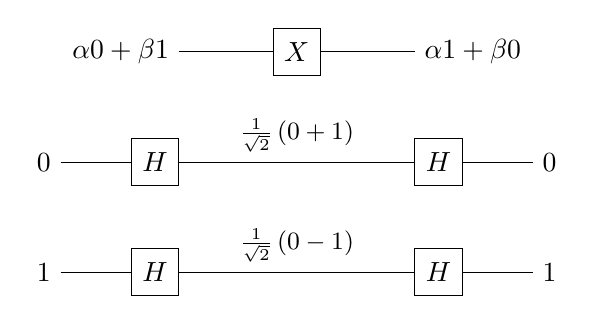
\begin{tikzpicture}[
            gate/.style={draw, fill=white, minimum size=6mm, inner sep=1pt},
        ]
        % X gate
        \draw (1.5,2.8) -- (4.5,2.8);
        \node[left] at (1.5,2.8) {$\alpha\ket{0} + \beta\ket{1}$};
        \node[gate] at (3,2.8) {$X$};
        \node[right] at (4.5,2.8) {$\alpha\ket{1} + \beta\ket{0}$};
        % H applied twice to |0> and to |1>
        \draw (0,1.4) -- (6,1.4);
        \node[left] at (0,1.4) {$\ket{0}$};
        \node[gate] at (1.2,1.4) {$H$};
        \node[above] at (3,1.4) {\small $\frac{1}{\sqrt{2}}\left(\ket{0} + \ket{1}\right)$};
        \node[gate] at (4.8,1.4) {$H$};
        \node[right] at (6,1.4) {$\ket{0}$};
        \draw (0,0) -- (6,0);
        \node[left] at (0,0) {$\ket{1}$};
        \node[gate] at (1.2,0) {$H$};
        \node[above] at (3,0) {\small $\frac{1}{\sqrt{2}}\left(\ket{0} - \ket{1}\right)$};
        \node[gate] at (4.8,0) {$H$};
        \node[right] at (6,0) {$\ket{1}$};
    \end{tikzpicture}
    \caption{One-qubit circuits. Top: the $X$ gate. Below: the Hadamard gate applied twice gives
        back the input, since $H^2 = I$ (\cref{lem:hh-0915}).}
    \label{fig:xh-0915}
\end{figure}

\section{The CNOT Gate}

\begin{definition}[CNOT Gate]\label{def:cnot-0915}
    The \textbf{controlled-NOT gate} (CNOT) is the two-qubit gate that maps the basis states by
    \[\ket{a} \ket{b} \longmapsto \ket{a} \ket{b \oplus a}, \qquad a, b \in \set{0,1},\]
    where $\oplus$ is XOR (addition modulo $2$). The first qubit $\ket{a}$ is the \textbf{control}
    qubit and is left unchanged; the second qubit $\ket{b}$ is the \textbf{target} qubit and is flipped
    exactly when $a = 1$. See \cref{fig:cnot-0915}.
\end{definition}

\begin{figure}[ht]
    \centering
    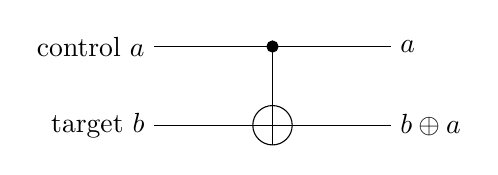
\begin{tikzpicture}
        \draw (0,1) -- (3,1);
        \draw (0,0) -- (3,0);
        \node[left] at (0,1) {control $\ket{a}$};
        \node[left] at (0,0) {target $\ket{b}$};
        \filldraw (1.5,1) circle (2pt);
        \draw (1.5,1) -- (1.5,-0.25);
        \draw (1.5,0) circle (0.25);
        \node[right] at (3,1) {$\ket{a}$};
        \node[right] at (3,0) {$\ket{b \oplus a}$};
    \end{tikzpicture}
    \caption{The CNOT gate: a filled dot on the control qubit and $\oplus$ on the target qubit.}
    \label{fig:cnot-0915}
\end{figure}

The four basis states are mapped as follows (for example $a = 1$, $b = 1$ gives $b \oplus a = 0$):
\[\begin{array}{c|cccc}
        \ket{a b}          & \ket{00} & \ket{01} & \ket{10} & \ket{11} \\ \hline
        \ket{a, b \oplus a} & \ket{00} & \ket{01} & \ket{11} & \ket{10}
    \end{array}\]

\begin{lemma}[Matrix of the CNOT Gate]\label{lem:cnot-0915}
    The matrix of the CNOT gate, with rows and columns indexed by $00, 01, 10, 11$, is the
    permutation matrix
    \[U_{\mathrm{CNOT}} = \begin{pmatrix}
            1 & 0 & 0 & 0 \\
            0 & 1 & 0 & 0 \\
            0 & 0 & 0 & 1 \\
            0 & 0 & 1 & 0
        \end{pmatrix}.\]
    It is unitary.
\end{lemma}

\begin{proof}
    The columns of the matrix of a gate are the images of the basis states. By the table, the images
    of $\ket{00}, \ket{01}, \ket{10}, \ket{11}$ are $\ket{00}, \ket{01}, \ket{11}, \ket{10}$, i.e., the
    column vectors
    \[\begin{pmatrix} 1 \\ 0 \\ 0 \\ 0 \end{pmatrix}, \quad
        \begin{pmatrix} 0 \\ 1 \\ 0 \\ 0 \end{pmatrix}, \quad
        \begin{pmatrix} 0 \\ 0 \\ 0 \\ 1 \end{pmatrix}, \quad
        \begin{pmatrix} 0 \\ 0 \\ 1 \\ 0 \end{pmatrix},\]
    which are the four columns of $U_{\mathrm{CNOT}}$, in this order.

    The map $\pi \colon (a, b) \mapsto (a, b \oplus a)$ on $\set{0,1}^2$ is its own inverse, since
    $\pi(\pi(a, b)) = (a, b \oplus a \oplus a) = (a, b)$. Hence $\pi$ is a bijection, i.e., a
    permutation of the four basis states, and $U_{\mathrm{CNOT}}$ is a \emph{permutation matrix}: every
    column is a standard basis vector, and different columns are different basis vectors.

    Every permutation matrix $P$ is unitary. The $(j, k)$ entry of $P^T P$ is the inner product of the
    $\nth{j}$ and the $\nth{k}$ column of $P$. These columns are standard basis vectors, equal if
    $j = k$ and different if $j \neq k$, so the entry is $1$ if $j = k$ and $0$ otherwise. Thus
    $P^T P = I$, and since $P$ is real, $P^\dagger P = P^T P = I$.
\end{proof}

In block form, $U_{\mathrm{CNOT}} = \begin{pmatrix} I & 0 \\ 0 & X \end{pmatrix}$: if the control is
$0$ (first two rows and columns) nothing happens, and if it is $1$ the gate $X$ is applied to the target.

\subsection{Classical Gates Are Not Reversible}

By \cref{thm:unitary-0915} and the remark after it, every quantum gate is unitary and therefore
invertible: the computation can be undone by applying $U^\dagger$. Classical gates such as AND, OR and
XOR, which take two bits to one bit, are \emph{not bijective}, hence \emph{not reversible}, hence
\emph{not unitary}. (Some classical gates, such as NOT, are reversible; the statement is about gates
that lose information.)

\begin{lemma}[XOR Is Not Reversible]\label{lem:xor-0915}
    The classical gate $\mathrm{XOR} \colon \set{0,1}^2 \to \set{0,1}$, $(a, b) \mapsto a \oplus b$, is
    not injective, so its input cannot be recovered from its output. The linear map
    $T \colon \mathbb{C}^4 \to \mathbb{C}^2$ with $T \ket{a b} = \ket{a \oplus b}$ does not preserve
    norms, so it is not unitary. The same holds for every gate with two input bits and one output bit.
\end{lemma}

\begin{proof}
    $\mathrm{XOR}(0,0) = 0 = \mathrm{XOR}(1,1)$, so two different inputs have the same output, and no
    function of the output can return the input in both cases. For the linear map,
    $T\left(\ket{00} - \ket{11}\right) = \ket{0} - \ket{0} = 0$, although
    $\norm{\ket{00} - \ket{11}} = \sqrt{2} \neq 0$. For a general gate $g \colon \set{0,1}^2 \to \set{0,1}$ there are four inputs and only two
    outputs, so by the pigeonhole principle two inputs $u \neq v$ have $g(u) = g(v)$, and the same
    argument applies with $\ket{u} - \ket{v}$. (For AND, take $u = 00$ and $v = 01$; for OR, $u = 01$
    and $v = 11$.)
\end{proof}

The CNOT gate is the reversible version of XOR: it computes $b \oplus a$ on the target wire, but it
also keeps a copy of $a$ on the control wire, and from $(a, b \oplus a)$ we recover
$b = (b \oplus a) \oplus a$. The example written in red in the notes and drawn on the board is the collision of XOR: the inputs
$00$ and $11$ give the same output $0$. In contrast, CNOT maps $\ket{00}$ to $\ket{00}$ and $\ket{11}$
to $\ket{10}$, two different outputs.

\section{Tensor Products and Entanglement}

The state of two qubits is built from the states of the single qubits by the tensor product.

\begin{definition}[Tensor Product]\label{def:tensor-0915}
    Let $A = (a_{ij})$ be an $m \times n$ matrix and let $B$ be a $p \times q$ matrix. The
    \textbf{tensor product} (Kronecker product) $A \otimes B$ is the $mp \times nq$ block matrix
    \[A \otimes B = \begin{pmatrix}
            a_{11} B & a_{12} B & \cdots & a_{1n} B \\
            a_{21} B & a_{22} B & \cdots & a_{2n} B \\
            \vdots   &          &        & \vdots   \\
            a_{m1} B & a_{m2} B & \cdots & a_{mn} B
        \end{pmatrix}.\]
    Column vectors are matrices with one column, so in particular
    \[\begin{pmatrix} \alpha \\ \beta \end{pmatrix} \otimes \begin{pmatrix} \gamma \\ \delta \end{pmatrix}
        = \begin{pmatrix} \alpha\gamma \\ \alpha\delta \\ \beta\gamma \\ \beta\delta \end{pmatrix}.\]
\end{definition}

For basis states this gives, for example,
$\ket{0} \otimes \ket{0} = (1, 0, 0, 0)^T = \ket{00}$ and
$\ket{1} \otimes \ket{0} = (0, 0, 1, 0)^T = \ket{10}$, and in general
\[\ket{a} \ket{b} = \ket{a} \otimes \ket{b} = \ket{a b}, \qquad a, b \in \set{0,1};\]
the three ways of writing are used interchangeably. In terms of kets, the formula for two vectors reads
\[\left(\alpha \ket{0} + \beta \ket{1}\right) \otimes \left(\gamma \ket{0} + \delta \ket{1}\right)
    = \alpha\gamma \ket{00} + \alpha\delta \ket{01} + \beta\gamma \ket{10} + \beta\delta \ket{11},\]
i.e., the tensor product is multiplied out like a product of sums. Gates combine in the same way: if
$A$ is applied to the first qubit and $B$ to the second, the two-qubit gate is $A \otimes B$, and
\begin{equation}\label{eq:mixed-0915}
    (A \otimes B)\left(\ket{x} \otimes \ket{y}\right) = A \ket{x} \otimes B \ket{y}.
\end{equation}
Indeed, if $x_1, \dots, x_n$ are the entries of $\ket{x}$, then $\ket{x} \otimes \ket{y}$ consists of
the blocks $x_1 \ket{y}, \dots, x_n \ket{y}$, so the $\nth{i}$ block of the left-hand side is
$\sum_{j} a_{ij} B \left(x_j \ket{y}\right) = \left(\sum_j a_{ij} x_j\right) B \ket{y}$, which is the
$\nth{i}$ block of the right-hand side.

\begin{definition}[Product State, Entangled State]
    A two-qubit state $\ket{\psi}$ is a \textbf{product state} if
    $\ket{\psi} = \ket{\phi_1} \otimes \ket{\phi_2}$ for some one-qubit states $\ket{\phi_1}$,
    $\ket{\phi_2}$. Otherwise $\ket{\psi}$ is \textbf{entangled}.
\end{definition}

In a product state each qubit has a state of its own. This is not always the case: the two qubits of
the \emph{Bell state} $\frac{1}{\sqrt{2}} \ket{00} + \frac{1}{\sqrt{2}} \ket{11}$ are entangled.

% Notes p. 10 (board): "1/sqrt2 |00> + 1/sqrt2 |11>  =/=  |alpha>|beta>", annotated "entangled
% qubits"; stated without proof.
\begin{exercise}\label{ex:bell-0915}
    Show that $\frac{1}{\sqrt{2}} \ket{00} + \frac{1}{\sqrt{2}} \ket{11} \neq \ket{\alpha} \ket{\beta}$
    for all one-qubit states $\ket{\alpha}$, $\ket{\beta}$.
\end{exercise}

The solution is \cref{thm:bell-0915}.

\begin{theorem}[The Bell State Is Entangled]\label{thm:bell-0915}
    The state $\frac{1}{\sqrt{2}} \ket{00} + \frac{1}{\sqrt{2}} \ket{11}$ is not a product state:
    there are no vectors $\ket{\phi_1}, \ket{\phi_2} \in \mathbb{C}^2$ with
    \[\frac{1}{\sqrt{2}} \ket{00} + \frac{1}{\sqrt{2}} \ket{11} = \ket{\phi_1} \otimes \ket{\phi_2}.\]
\end{theorem}

\begin{proof}
    Suppose there are, and write $\ket{\phi_1} = \begin{pmatrix} \alpha \\ \beta \end{pmatrix}$ and
    $\ket{\phi_2} = \begin{pmatrix} \gamma \\ \delta \end{pmatrix}$. By \cref{def:tensor-0915},
    comparing the four entries of the two sides gives
    \[\alpha\gamma = \frac{1}{\sqrt{2}}, \qquad \alpha\delta = 0, \qquad \beta\gamma = 0,
        \qquad \beta\delta = \frac{1}{\sqrt{2}}.\]
    From $\alpha\delta = 0$ we get $\alpha = 0$ or $\delta = 0$. If $\alpha = 0$ then
    $\alpha\gamma = 0 \neq \sfrac{1}{\sqrt{2}}$, and if $\delta = 0$ then
    $\beta\delta = 0 \neq \sfrac{1}{\sqrt{2}}$. Both cases are contradictions.
\end{proof}
